\documentclass[../main.tex]{subfiles}

\begin{document}

\section{Operations, Primitives and Algorithms}
The following sections introduce, define and explain Operations, Primitives and Algorithms generally using the Terminology presented below. Operations are the building blocks of Primitives whereas Primitives are the building blocks of Algorithms. The definitions which follow are flexible enough to support implementation across programing languages but have been inspired by the core concepts found within Lisp. The focus of these sections is to define the properties of and interactions between Operations, Primitives and Algorithms in a general way which doesn't place unnecessary bounds on their range of possible functionality with respect to processing xAPI data.

\subsection{Terminology}

In the subsections and sections which follow, (s) indicates one or more

\subsubsection{Scalar}

Singular value $x$ of a fundamental JSON type as described by \href{https://json-schema.org/understanding-json-schema/reference/type.html}{JSON Schema}

\subsubsection{Collection}

a n-tuple of items $x$ such that
$$X = <x_{i}..x_{n}..x_{j}>$$

where
$$i \leq n \leq j \implies i \prec n \prec j \iff i \not= n \not= j$$

\subsubsection{Key}

A lookup $k$ for a $v$ within a $kv$ where $k = x \lor X$

\subsubsection{Value}

a piece of data $v$ where $v = x \lor X$

\subsubsection{Key Value pair}

Association between a $k$ and $v$ where
$$k \mapsto v$$

such that
$$kv = k \mapsto v$$
and a collection of Key Value pair(s) is defined as
$$KV = <kv_{i}..kv_{n}..kv_{j}>$$

such that
$$ k_{n} \mapsto v_{n}$$

and all $k$ within $KV$ are unique
$$i_{k} \not= n_{k} \not= j_{k} $$

but the same is not true for all $v$ within $KV$
$$i_{v} = n_{v} \lor i_{v} \not= n_{v} \
i_{v} = j_{v} \lor i_{v} \not= j_{v} \
j_{v} = n_{v} \lor j_{v} \not= n_{v}$$

\subsubsection{Statement}

Immutable collection of Key Value Pair(s) conforming to the \href{https://github.com/adlnet/xAPI-Spec/blob/master/xAPI-Data.md#24-statement-properties}{xAPI Specification}

\subsubsection{Algorithm State}

Mutable collection of Key Value Pair(s)

\subsubsection{Option}

Collection of Key Value Pair(s) which alter the result of an Algorithm

\subsection{Operation}

Given an input X, an Operation produces output Y
$\\\\$
{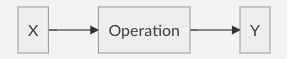
\includegraphics[page=1]{operation-x}}
$\\\\$
If X changes to X' then the Operation results in Y' instead of Y
$\\\\$
{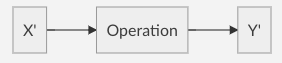
\includegraphics[page=1]{operation-x-prime}}

\subsubsection{Domain}

Any of the following
\begin{itemize}
\item Key(s)
\item Value(s)
\item Key Value pair(s)
\item Statement(s)
\item Algorithm State
\end{itemize}

\subsubsection{Range}

Any of the following dependent upon the Domain and Functionality of the Operation

\begin{itemize}
\item Key(s)
\item Value(s)
\item Key Value pair(s)
\item Statement(s)
\item Algorithm State
\end{itemize}

\subsubsection{Formal Definition}

A relationship between input and output data which will result in the same $Y$ given the same $X$

$$Operation(X) = Y \land \ Operation(X') = Y'$$
$$\implies$$
$$Y = Y' \iff X = X'  \land Y \not= Y' \iff X \not= X'$$
When $X$ is a collection, that collection consists of one or more members $x_{n}$ within the range $i..j$ such that
$$i \leq n \leq j  \implies i \prec n \prec j \iff i \not= n \not= j$$
which allows collection $X$ to be defined as
$$X = <x_{i}..x_{n}..x_{j}> $$
and the output of $Operation(X)$ to be defined as
$$Y = <y_{i}..y_{n}..y_{j}>$$
such that the mapping from $Operation(X) \to Y$ can be defined as
$$Operation(x_{i}) \mapsto y_{i} \land Operation(x_{n}) \mapsto y_{n} \land Operation(x_{j}) \mapsto y_{j}$$
which implies that the collection $Y$ has the same ordering as collection $X$
$$ i_{Operation(x)} = i_{y} \ \land \ n_{Operation(x)} = n_{y} \ \land \ j_{Operation(x)} = j_{y} $$
and allows us to define the $input \to output$ relationship of an $Operation$ in terms of collection members
$$Operation(x) = y$$
which establishes how an $Operation$ responds to non-distinct values within a Collection
$$Operation(x_{n}) = y_{n}$$
$$Operation(x_{n'}) = y_{n'}$$
$$Operation(x_{n' + 1}) = y_{n'}$$
$$\iff$$
$$x_{n'} \equiv x_{n'+1} \land x_{n'} \not \equiv x_{n}$$
$$\implies $$
$$x_{n} \not \equiv  x_{n' + 1}$$
$$\implies $$
$$Operation(x_{n'}) = Operation(x_{n' + 1}) \not= Operation(x_{n})$$

\end{document}
